\documentclass[12pt]{amsart}

    \addtolength{\hoffset}{-2.25cm}
    \addtolength{\textwidth}{4.5cm}
    \addtolength{\voffset}{-2.5cm}
    \addtolength{\textheight}{5cm}
    \setlength{\parskip}{0pt}
    \setlength{\parindent}{15pt}
    
    \usepackage{amsthm}
    \usepackage{textcomp}
    \usepackage{amsmath}
    \usepackage{amssymb}
    \usepackage[utf8]{inputenc}
    \usepackage[colorlinks = true, linkcolor = black, citecolor = black, final]{hyperref}
    
    \usepackage{graphicx}
    \graphicspath{ {images/} }
    \usepackage{multicol}
    \usepackage{ marvosym }
    \usepackage{wasysym}
    \usepackage{tikz}
    \usetikzlibrary{patterns}
    
    \newcommand{\ds}{\displaystyle}
    \DeclareMathOperator{\sech}{sech}
    
    
    \setlength{\parindent}{0in}
    \pagestyle{empty}
    \begin{document}
    \thispagestyle{empty}
    {\scshape Nacchofer31} \hfill {\scshape \large Apuntes MFI} \hfill {\scshape Tema \#1}
     
    \hrule
    \medskip
    
    \textbf{- La lógica}, proporciona una formulación \textbf{simbólica} e \textbf{independiente del dominio} de las leyes del pensamiento humano.
    Este doble carácter hace posible mecanizar sus técnicas y métodos. 
    
    \begin{itemize}
    
    \item  PROBLEMA: 
    
    - Tiene un carácter \textbf{estático}, se desarrolló para estudiar objetos matemáticos  bien definidos y consistentes, se requieren
    formas más dinámicas (y menos perfectas) de lógica. 
    
    - Los métodos de la lógica resultan más \textbf{caros} en términos computacionales, es necesario reducir sus costes.
    \item  SOLUCIÓN: \textbf{Lógica computacional}, modela el conocimiento impreciso, incompleto, dinámico, distribuido. 
    Soporta el razonamiento aproximado, temporal, no monótono,...
    
    
    \end{itemize}
    
    \textbf{Lógicas para Aplicaciones software:}

    
    
    Restricciones: \emph{- Lógica ecuacional}
    
    Extensiones de la lógica: \emph{- Lógica difusa - Lógica Lineal - Lógica
    Modales}

    \textbf{- Lógica ecuacional:}
    
    \begin{itemize}
    
    \item  Subconjunto de la lógica de primer orden,
     se eliminan todas las conectivas lógicas. El símbolo de predicado
     es la (=).
    \item s=t, dos términos son semánticamente iguales, aunque son diferentes
     sintácticamente. \emph{Ej: ascii('0') = 48}
    \item Un conjunto E de ecuaciones con el mismo símbolo "raíz" f
    en las partes izquierdas de las ecuaciones se describe como
    "la definición" de f. \emph{even(0)=true - even(X)=even(X-2)}
    
    \end{itemize}
    
    \textbf{Lógica para la programación:}

    Restricciones - Estilo de Lenguaje: 
    
    - \emph{Lógica ecuacional - Funcional (Haskell)}
    
    - \emph{Lógica clasual - Relacional (Prolog)}
    
    Extensiones: 
    
    - \emph{Lógica many-sorted +tipos}

    - \emph{Lógica order-sorted +herencia}

    - \emph{Lógica (modal) temporal +concurrencia}

    - \emph{Lógica (modal) dinámica +objetos}
    
    \textbf{- Unificación de lógicas: Lógica de Reescritura (RWL)}, 
    lógica del cambio que permite especificar la dinámica de un
    sistema. 
    
    \begin{itemize}
    
    \item  Integración "sin costuras" de distintas características: funciones,
    y tipos, indeterminismo, concurrencia, reflexión y genericidad.
    
    \item  Marco unificado en el que pueden definir distintas lógicas: ecuacional, clasual, lineal.
    
    \item  Existe una lógica temporal, asociada a la RWL, estrictamente
    más potente que CTL/LTL: la temporal logic of rewriting (LTR).
    
    \end{itemize}
    
    \textbf{- Maude:}, implementa eficientemente la lógica
    RWL.  
     \begin{itemize}
    
        \item Soporta de forma natural la especificación formal / modelado
        / programación en un estilo funcional.
        
        \item  Distingue entre la parte concurrente y funcional.
        
        \item  Reescritura módulo listas, conjuntos, multiconjuntos,...
        mediante atributos ecuacionales.

        \item Genericidad y tipos ordenados de datos.

        \item Infraestructura para análisis y verficación formal
        (alcanzabilidad, model-checking, theorem proving).

        \item Reflexión como soporte al meta-modelado, ejecución
        simbólica y construcción rápida de herramientas de soporte.
        
        \end{itemize}
    \pagebreak

    \textbf{- Lenguaje Maude}

    \begin{itemize}
        \item Sintaxis: Basada en ecuaciones y reglas de reescritura
        (estilo Haskell, ML, Scheme o Lisp)
        \item Semántica: Basada en la Lógica de Reescritura (RWL), que
        modela funciones, concurrencia y objetos.
    \end{itemize}

    \textbf{- Fundamentos de Maude}, consta de tres tipos de módulos:

    \begin{itemize}
        \item Módulos funcionales \emph{fmod \textless conjunto de ecuaciones \textgreater endfm}
        \item Módulos de sistema \emph{mod \textless conjunto de ecuaciones/reglas de escritura \textgreater endm}
        \item Módulos O2 \emph{omod ... endom}
    \end{itemize}

    \textbf{- E (Ecuaciones):}
    \begin{itemize}
        \item Definen funciones confluentes y terminantes.
        \item Se definen dentro de módulos funcionales.
        \item E puede incluir un conjunto Ax de Axiomas algebraicos.
        \item Representan la parte estática del sistema.
        \item Se aplican de forma determinista.
    \end{itemize}

    \textbf{- R (Reglas de reescritura):}
    \begin{itemize}
        \item Definen funciones que pueden ser no confluentes y/o no
        terminantes.
        \item Se definen dentro de módulos de sistema.
        \item Especifican la dinámica del sistema, es decir, acciones que
        puedan producir transiciones del mismo.
    \end{itemize}

    \textbf{- Paso de reescritura (Maude step)}, dado un término (o estado) s,
    un paso de reescritura de t a t' se consigue aplicando una regla de R
    módulo las ecuaciones de E. 

    El estado t se simplifica usando las ecuaciones de E hasta
    alcanzar su forma irreducible (tE) con respecto E.

    Una traza de ejecución es una secuencia de Maude steps.
    Se representa como: t ----- \textgreater t'

    \textbf{- Reescritura módulos axiomas}, dado E=Eo U Ax,
    las ecuaciones de Ax no se usan para reescribir sino
    para hacer un pattern-matching especializado. Cuando el
    conjunto de axiomas algebraicos no es vacio, cada paso
    de reescritura se hace sustituyendo el pattern-matching
    convencional por pattern-matching módulo axiomas.

    \textbf{- Árbol de ejecución}, un árbol de computación
    es un conjunto de secuencias de Maude steps que se organizan en
    forma de árbol.

    \textbf{- Optimización}, Maude mantiene en memoria versiones
    normalizadas de las reglas y ecuaciones del programa, donde sus
    lh's están normalizadas respecto de Ax. 
    
    En cada Maude step, la fase inicial se descompone en dos normalizaciones,
    la primera respecto a los axiomas de Ax y la segunda respecto de
    las ecuaciones de Eo.

    \textbf{- Atributos ecuacionales}, cuando aparecen operadores con
    axiomas asociativos, conmutativos, etc, la reescritura no es capaz
    de computar de forma efectiva con ellos (espacio de búsqueda
    infinito). Para ello, dichas propiedades se tratan aparte, como
    \textbf{atributos}.

    \medskip

    pares no ordenados --- \textgreater comm \emph{XY=YX}

    listas --- \textgreater assoc \emph{X(YZ) = (XY)Z} --- id:null 
    \emph{Xnull = nullX = X}

    multiconjuntos --- \textgreater assoc, comm, id:null

    conjuntos --- \textgreater assoc, comm, id:null, idem \emph{XX = X}
    
    \textbf{[assoc idem] PROHIBIDO EN MAUDE}

    \medskip

    \textbf{- Otros atributos ecuacionales}

    - [ctor] --- \textgreater símbolo constructor
    
    - [gather (e E)] --- \textgreater assoc por la derecha

    - [item] --- \textgreater abrevia s(s(..(0))) como sn(0)

    - [ditto] --- \textgreater mismos axiomas que el anterior

    \textbf{- Ecuaciones}, se usan para normalizar los estados.
    \textbf{Reglas,} se usan para hacer evolucionar el sistema
    produciendo cambios de estado.

    \textbf{- Estrategias de evaluación}, a diferencia de otros
    lenguajes funcionales como Haskell, que son perezosos, Maude es
    un lenguaje impaciente (sólo para las ecuaciones).

    Para garantizar la convegencia y terminación de los cómputos, es
    necesario que las ecuaciones satisfagan buenas condiciones.

    \textbf{- Terminación}, un programa es terminante si no existen
    cadenas infinitas de pasos de reducción. Cuando un programa
    es terminante, la forma normal de cualquier término siempre existe.
    
    La terminación es una propiedad indecidible de los programas.

    \textbf{- Confluencia}, un programa es confluente si, siempre
    que un término se puede reescribir a dos términos distintos,
    éstos, a su vez, convergen a un mismo término.

    \textbf{- Ortogonalidad --- \textgreater Confluencia}, cuando un
    programa es confluente, la forma normal de cualquier término,
    si existe, es única. 
    \begin{itemize}
        \item La confluencia es indecidible.
        \item Hay condiciones suficientes. Ej: la ortogonalidad donde
        Ortogonalidad = no solapamiento de lh's (ninguna instancia en común)
         + linealidad por la izquierda (no variables repetidas)
    \end{itemize}

    \textbf{- Reescritura condicional}, las reglas/ecuaciones
    condicionales tienen la forma general: 
    \begin{itemize}
        \item crl l = \textgreater r if C
        \item ceq l = \textgreater r if C
    \end{itemize}

    Donde C es una conjunción de expresiones del tipo: \emph{equation,
    matching equation, sort expression, rule}.
    
    \textbf{- Lógica Fuzzy (borrosa, difusa) - Extensiones de la lógica},
    soporta el razonamiento aproximado (útil en robótica, sistemas expertos,...).
    \begin{itemize}
        \item Multivaluada, en vez de binaria, que se deriva -o es una
        aplicación- de la teoría de "conjuntos Fuzzy", (valores entre 0 y 1)
        \item Ejemplos: Lukasiewicz, Goedel, Pavelka.
    \end{itemize}

    \textbf{- Lógica Lineal (Girald, 1987) - Extensiones de la lógica},
    permite actualizar la cantidad de recursos tras cada cambio de estado 
    (útil en control de recursos)

    \begin{itemize}
        \item La implicación en lógica lineal se escribe ---o y se llama "lolli"
        \item En dicha implicación, se consume el recurso A para producir
        B, las condiciones se modifican tras su uso, es decir, los recursos
        se consumen al usarlos.
        \item Nuevas conectivas lógicas: ! of course (replicación), ? why not (borrado)
        \item Separación en dos clases de las conectivas estándar: "multiplicativa"
        o simultánea, y otra "aditiva".
        \item La conjunción \& es una conjunción ya que se puede probar
        simultáneamente y no es una disyunción. 
    \end{itemize}

    \textbf{- Lógica Modal - Extensiones de la lógica}, nuevos cuantificadores
    (modales):
    \begin{itemize}
        \item  Temporales: UNIVERSAL always, EXISTENCIAL sometimes para formalizar el tiempo,
        creencias,...
        \item Dinámicas: Lógicas de la acción: lógica modal para razonar
        acerca de las acciones y procesos.
        \item Epistémicas: Lógicas del Conocimiento y de la Creencia/Ignorancia.
    \end{itemize}

    \textbf{- Lógica del Tiempo}, se desarrollaron por los filósofos
    para investigar cómo el tiempo se usa en el lenguaje natural
    de las personas.

    Superan la aproximación de primer orden, donde lo habitual es introducir un simple argumento extra para el tiempo.

    \textbf{- Aproximaciones rivales}, las dos aproximaciones, clásica y
    temporal, son rivales.

    En terminología de BDs:
    
    \begin{itemize}
        \item  \emph{tensers}, son partidarios de la
        aproximación modal temporal.

        \item \emph{detenser}, partidarios de la aproximación de primer
        orden.

    \end{itemize}
    
    {\scshape Nacchofer31} \hfill {\scshape \large Apuntes MFI} \hfill {\scshape Tema \#2}
     
    \hrule
    \medskip
    
    \textbf{- La Trilogía del Software}, consta de los siguientes
    componentes de software:
    
    \begin{itemize}
        \item \textbf{Propiedades}: Especificaciones, requerimientos,
        tipos, modelos (grafos, fórmulas).
        \item \textbf{Juegos de datos}: Seq: trazas, Out: Escenarios,
        In: Ejemplos 
        \item \textbf{Programas}: Código, documentación, Proofs.
    \end{itemize}
    
    \textbf{- Procesos Formales de la Trilogía:}

    Propiedades a Programas: Derivación formal

    Programas a Propiedades: Model checking. Análisis y verficación automática
    del Software.

    Propiedades a Propiedades: Transformación de modelos. Programación
    automática.

    Programas a Programas: Transformación de programas. Especialización,
    Fragmentación, Refactorización.

    Datos a Datos: Minería de datos.

    Programas/Propiedades a Datos: Generación automática de casos de
    prueba.
    
    Datos a Programas/Propiedades: Aprendizaje automático de programas/
    propiedades a partir de Ejemplos.

    \textbf{- Hiperprocesos en la Trilogía}

    \begin{itemize}
        \item Depuración/Diagnóstico Racional/
        Declarativo
        \item Model Checking 
        \item Certificación de Programas
    \end{itemize}

    \textbf{- De Propiedades a Programas}

    \begin{itemize}
        \item \textrightarrow Derivación Formal de programas
        \item \textrightarrow Programación automática (a
        gran escala)
    \end{itemize}

    \textbf{- De Propiedades a Programas (y viceversa)}

    \begin{itemize}
        \item \textrightarrow Derivación Formal de programas
        \item \textleftarrow Verificación Formal 
        \item \textleftarrow Type interface
        \item \textleftarrow Síntesis de Especificaciones a
        partir de programas
    \end{itemize}
    \begin{center}
        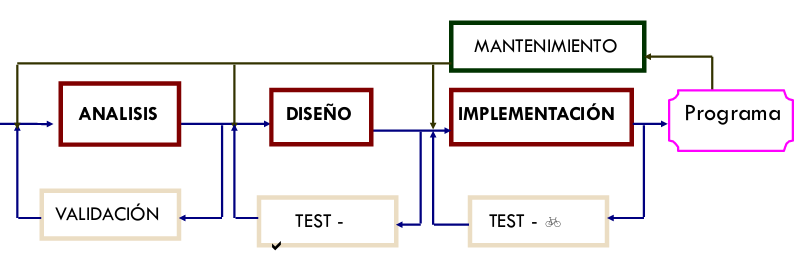
\includegraphics[width=10cm, height=5cm]{t2clasico.png}
        
        Ciclo de Vida Clásico

        \medskip

        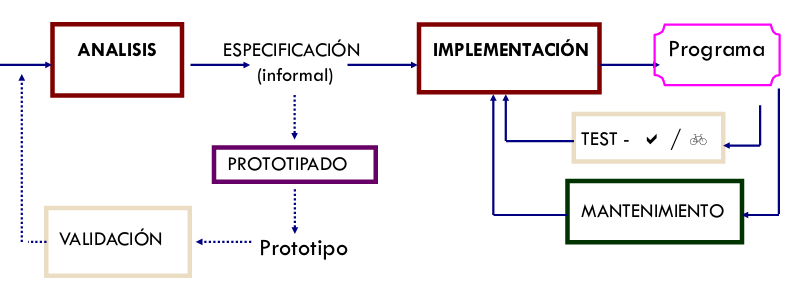
\includegraphics[width=10cm, height=5cm]{t2prototipo.png}
        
        Ciclo de Vida con Prototipado
    \end{center}
    
    \textbf{- De Propiedades a Propiedades}

    \begin{itemize}
        \item \textrightarrow Transformación de Modelos
        \item \textrightarrow Programación Automática
    \end{itemize}

    \begin{center}
        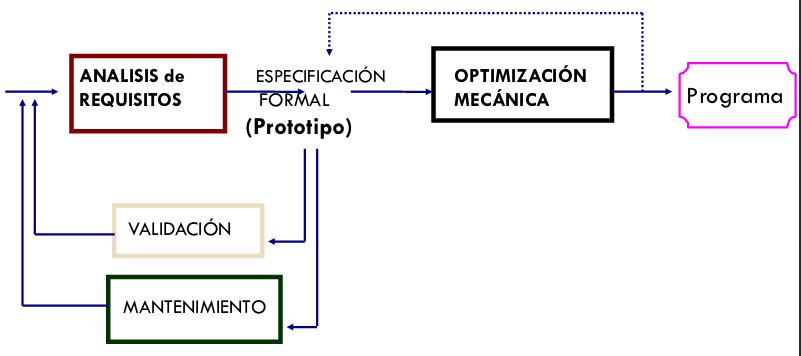
\includegraphics[width=10cm, height=5cm]{t2progauto.png}
        
        Programación Automática
    \end{center}

    

    
    \end{document}